\documentclass{article}
\usepackage[utf8x]{inputenc}
\usepackage[russian]{babel}
\usepackage [T2A] {fontenc}
\usepackage{amsmath,amsfonts,amssymb,amsthm}
\usepackage[left=20mm, top=20mm, right=20mm, bottom=20mm]{geometry}
\usepackage{amsmath}
\usepackage{graphicx}
\def\*#1{\mathbf{#1}}

\begin{document}
\author{Михаил Богомолов}
\title{Compressive Sensing Experiments}
\date{}
\maketitle

\section{Теория}.

Введём пару определений.

\textbf{Определение 1.} Назовём $k$-разреженным ($k$-sparse) вектор, который имеет $k$ ненулевых компонент.

\textbf{Определение 2.} Назовём сжимаемым (compressible) вектор, в котором отсортированные абсолютные значения компонент убывают по степенному закону (т.е. $k$-тая порядковая статистика мажорируется функцией $\cfrac{c}{k^\alpha}, \alpha > 0$).

Утверждается, что $\forall s, n\ \exists m \ll n$ и такая матрица $\*A$ размера $m \times n$, что по вектору $\*y = \*A\*x$ можно однозначно восстановить вектор $\*x$, если $\*x$ был $s$-разреженным.

То есть, решение задачи $||\*x||_0 \leq s, s.t.\ \*A\*x = \*y$ единственно. Однако в силу того, что минимизация $l_0$-псевдонормы --- NP-полная задача (эквивалентна \textsf{SUBSET-SUM}), уже для небольших $n$ решить исходную задачу не представляется возможным. Поэтому вместо такой задачи решается следующая:

$$||\*x||_1 \to \min, s.t.\ \*A\*x = \*y$$

В действительности оказывается, что это не только вычислительный трюк. Есть теорема, которая утверждает, что при некоторых условиях минимизация $l_1$-нормы даёт не просто приемлемый результат, а действительно точный.

Условие это такое:

Пусть существует такое $\delta_{s}$, что для любых $s$-разреженных векторов выполнено следующее условие:

$$(1 - \delta_{s}) ||\*x||_2^2 \leq ||\*A\*x||_2^2 \leq (1 + \delta_{s}) ||\*x||_2^2.$$

Тогда будем называть матрицу $\*A$ подчиняющейся restricted isometry property (RIP) порядка $s$ с константой $\delta_s$.

\textbf{Теорема.} Для того, чтобы минимизация $L_1$-нормы давала точное решение для всех $s$-разреженных векторов, требуется, чтобы $\*A$ подчинялось RIP порядка $3s$, и при этом $\delta_{2s} + \delta_{3s} < 1.$ 

Это довольно сложное условие, его тяжело просто так проверить. Однако для некоторых типов матриц (в основном, сгенерированных из некоторого случайного распределения) доказано, что они подчиняются RIP.

Например:

\begin{enumerate}
	\item Матрица размера $m \times n$, элементами которой являются i.i.d. гауссовские случайные величины c дисперсией $1/m$.
	\item I.i.d. случайные величины из распределения с двумя равновероятными значениями $\pm \cfrac{1}{\sqrt{m}}$.
	\item Случайные стобцы из базиса Фурье.
\end{enumerate}

Для первых двух матриц утверждается, что они удовлетворяют теореме с вероятностью $1 - O(e^{-\gamma n})$, если $s = O(m / \log(n/m))$ или $m = O(s \log(n/s))$. А значит, матрицы из i.i.d. гауссовских и бернуллиевских величин (с любыми матожиданиями и дисперсиями) хорошо подходят для compressive sensing.

Для третьего типа матриц утверждается, что они позволяют восстанавливать разреженный вектор, если $m = O(s (\log n)^4)$.

Первый тип матриц мне кажется особенно удачным для практического применения в анализе многих данных. Это связано с тем, что обычно данные представлены не в разреженном базисе, но существует некоторый ортогональный базис, в котором они разрежены. При этом произведение ортогональной матрицы и матрицы из i.i.d. гауссовских случайных величин даёт матрицу из того же распределения!

То есть: пусть $\Psi$ --- базис, в котором измерения являются разреженными, $\*s$ --- разреженный вектор измерений, $\*x = \Psi \*s$ --- наблюдаемый вектор измерений, $\Phi$ --- матрица из гауссовских случайных величин. Так как $\Phi \Psi$ --- тоже гауссовская матрица, то разреженное решение системы $\*y = \Phi \Psi \*s$ единственно, и совпадает с $\*s$.

Третий тип удачнее первых двух, поскольку он требует гораздо меньшего количества дополнительных данных ($O(n)$ против $O(mn)$). Его можно использовать для сжатой передачи информации.

\section{Что получилось сделать}

Я решил проверить, что сочетание удачной sensing matrix и минимизации $L_1$-нормы даёт хороший результат.

\subsection{Sparse vectors}

Я свёл задачу минимизации $L_1$-нормы к задаче линейного программирования. Исходная задача такая:

$$||\*x||_1 \to \min, s.t.\ \*A\*x = \*y.$$

Задача линейного программирования получается такая:
\begin{align*}
    &x_1+\cdots+x_n \to \min, \\
s.t.\    &\*A\*x = \*y, \\
    &-\*t \leq \*x \leq -\*t, \\
    &\*t \geq 0 \\
\end{align*}

Затем я брал различные типы sensing matrices, генерировал случайные $k$-разреженные вектора и подбирал бинпоиском минимальное значение $m$, что разность настоящего ответа и найденного решения отличается на малую величину.

Получившиеся результаты для различных типов матриц:

\begin{enumerate}
	\item Гауссовские случайные величины ($50 \leq n \leq 200$, $k \leq n$, $m$ подобрано).
	\begin{center}
	    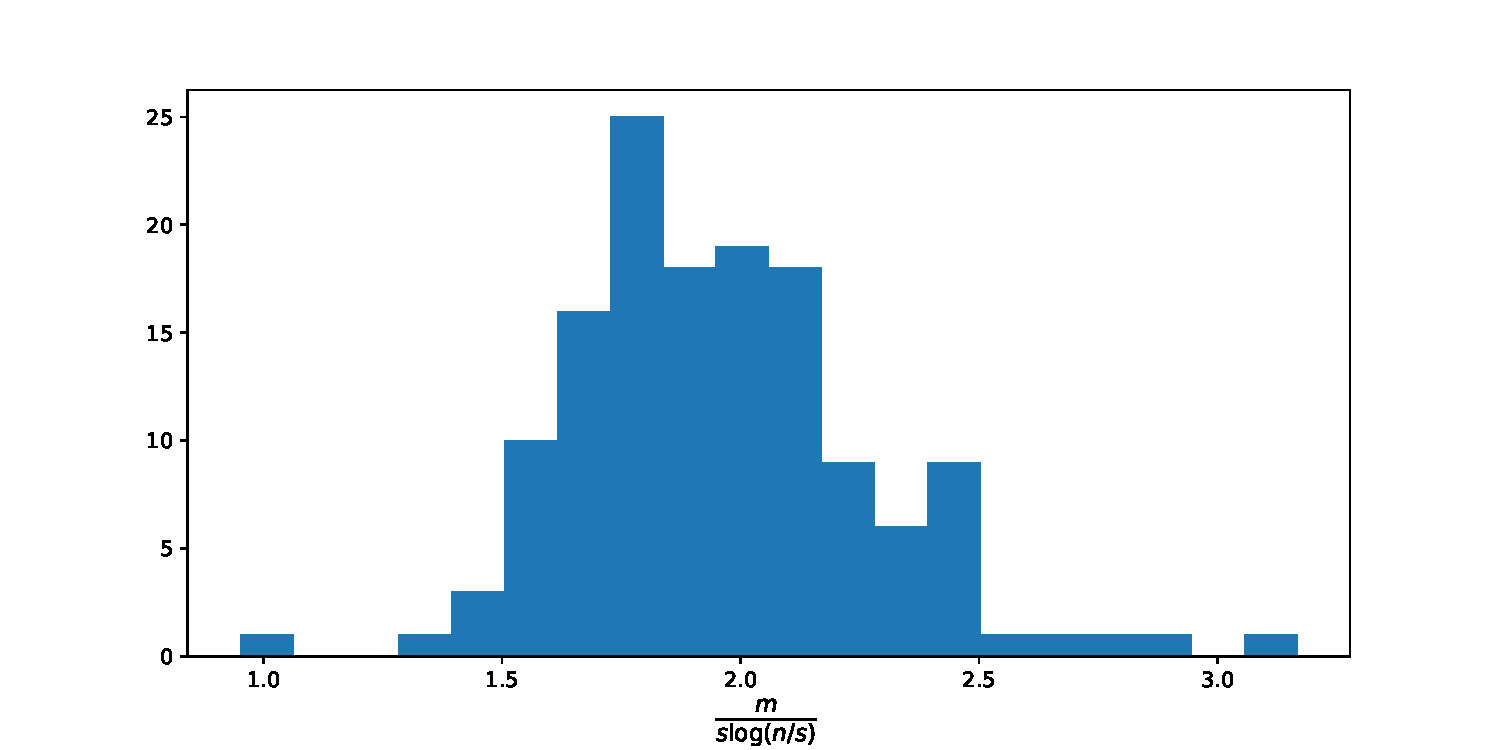
\includegraphics[scale=0.75]{gaussian}
    \end{center}
	
	\item Бернуллиевские случайные величины ($50 \leq n \leq 125$, $k \leq n$, $m$ подобрано).
	\begin{center}
	    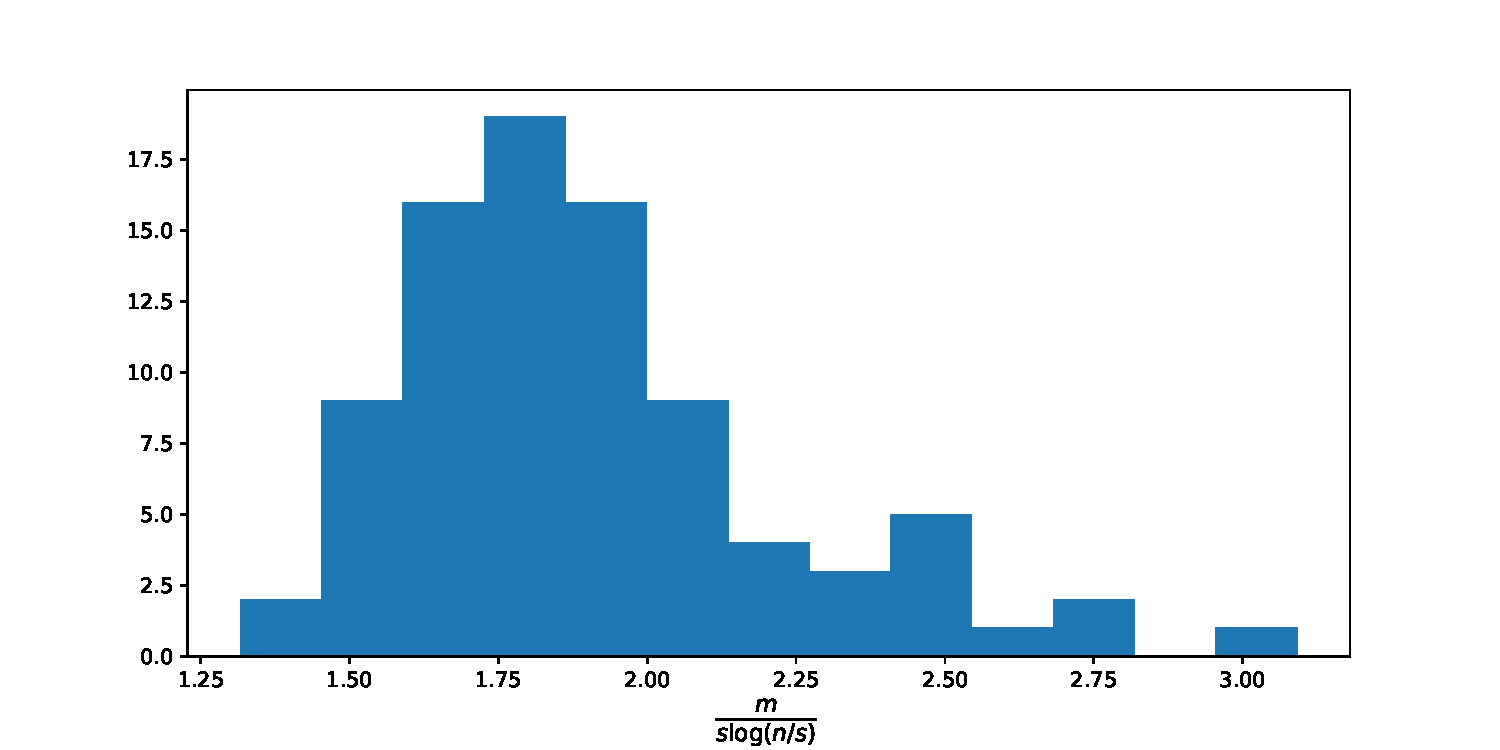
\includegraphics[scale=0.75]{bernoulli}
    \end{center}
    
    \item Рандомные столбцы из базиса Фурье ($50 \leq n \leq 125$, $k \leq n$, $m$ подобрано).
    \begin{center}
	    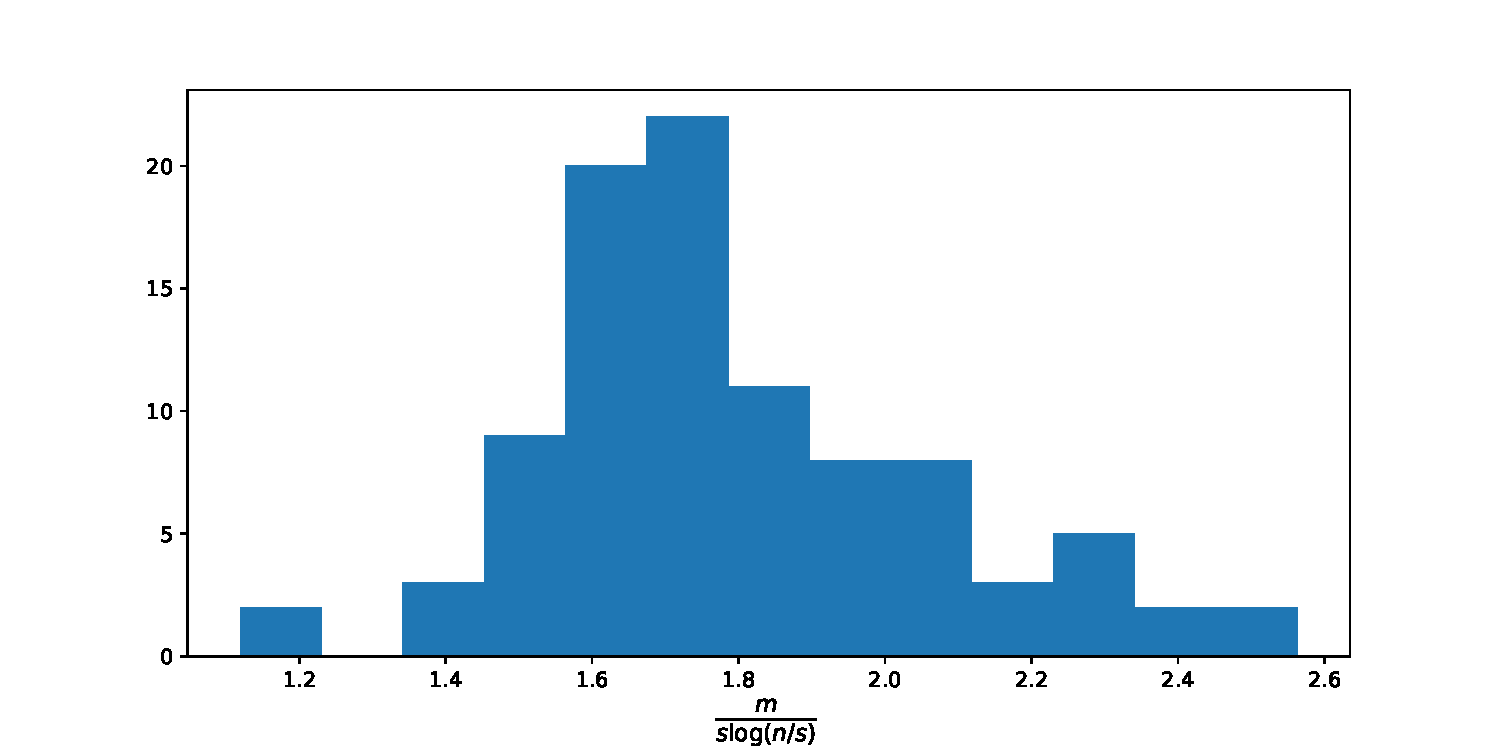
\includegraphics[scale=0.75]{fourier}
    \end{center}
\end{enumerate}

Вообще, для последнего типа sensing matrix нужно было проверять не $m = s \log(n/s)$, а $m = O(s (\log n)^4)$, что заметно хуже, но почему-то $m = s \log(n/s)$ тоже хорошо получилось. Возможно, это связано с тем, что оценка с четвертой степенью --- детерминированная оценка худшего случая, а я тестировал на случайных векторах. Но это всё равно здорово: получается, такой тип матриц не хуже полностью рандомных, при условии, что сами данные имеют случайное распределение.

%график, таблица для гауссовских, бернуллиевских, псевдослучайных бернуллиевских, chipping sequence, шахматной доски

\subsection{Compressive vectors}

Обычные данные, скорее, являются не разреженными, а сжимаемыми: в них кроме нескольких значимых компонент существует ещё много совсем небольших. Поэтому я решил ещё проверить, как хорошо можно восстановить такие вектора. Однако у меня не получилось восстанавливать эти небольшие компоненты точно. В случае разреженных векторов можно было использовать в качестве предиката в бинпоиске условие, что найденный вектор по норме отличается от истинного на малое постоянное значение $\varepsilon$ (например, $10^{-9}$). Когда я начал зашумлять разреженные данные на весьма малый гауссовский шум (со стандартным отклонением $\varepsilon~=~\cfrac{1}{cn}, c~>~1$), т.е. прибавлять к разреженному вектору $\*x$ гауссовский вектор $\*x_\varepsilon$, оказалось, что ни $\*x$, ни $\*x + \*x_\varepsilon$ восстановить нельзя, а в лучшем случае получается какой-то вектор, близкий к $\*x + \*x_\varepsilon$ и отличающийся от него по норме на что-то порядка $\varepsilon n / 10$ (не очень понимаю, почему такая константа, но близкие числа получались при различных значениях $n, m, k$).

Я пробовал разные способы восстановления зашумлённого разреженного вектора:

\begin{enumerate}
	\item Способ, описанный выше: простая минимизация $||\*x||_1$ при условии $\*A \*x = \*y$, где $\*x$ --- уже зашумленный вектор. Это не позволяет отделить шум, но об этом дальше.
	\item Модифицированный способ 1. 
	\begin{align*}
    &x_1+\cdots+x_n \to \min, \\
s.t.\    &\*y - 2\varepsilon \leq \*A\*x \leq \*y + 2\varepsilon, \\
    &-\*t \leq \*x \leq -\*t, \\
    &\*t \geq 0 \\
\end{align*}

    Идея этого метода была в том, чтобы искать такой вектор $\*x$ с маленькой нормой, чтобы $\*A \*x$ отклонялся от $\*y$ не слишком сильно.
    \item Однако $\*y$ в действительности часто мог отклоняться от нужного значения больше, чем на $2 \varepsilon$. Это происходило из-за того, что небольшое гауссовское отклонение по $\*x$ становилось довольно большим, из-за того, что в $\*A$ могли быть довольно большие сингулярные числа. Поэтому я решил воспользоваться сингулярным разложением, чтобы проконтролировать допустимую ошибку по $\*y$.
    
    Что я сделал: пусть $\*x$ зашумлён случайным гауссовским вектором $\*x_\varepsilon$ со стандартным отклонением $\varepsilon$. Пусть $\*A = \*U \*\Sigma \*V^\top$ --- сингулярное разложение. Заметим, что $\*V^\top \*x_\varepsilon$ --- тоже вектор i.i.d. гауссовских случайных величин со стандартным отклонением $\varepsilon$, т.к. $\*V^\top$ --- ортогональная матрица. При домножении гауссовского вектора независимых случайных величин на диагональную матрицу $\*\Sigma$ стандартные отклонения всех его компонент домножаются на соответствующие сингулярные числа. Получается вектор из независимых нормальных случайных величин со стандартными отклонениями, пропорциональными сингулярным числам. Будем решать следующую задачу:
    \begin{align*}
    &||x||_1 \to \min, \\
s.t.\    &\*U^\top\*y - 2\varepsilon\mathrm{diag}(\*\Sigma) \leq \*\Sigma\*V^\top\*x \leq \*U^\top\*y + 2\varepsilon\mathrm{diag}(\*\Sigma)
\end{align*}

    По сути это задача поиска такого вектора $\*x$ с минимальной $L_1$-нормой, что в его $2\varepsilon$-окрестности есть такой вектор, который при домножении на $\*A$ даёт известный $\*y$.
\end{enumerate}

    При подборе минимального размера $m$ для матрицы $\*A$ третий способ показал наилучшие результаты, но почему-то, во-первых, эти результаты были не сильно лучше первого, а во-вторых, восстановление исходного разреженного вектора всё равно не удавалось (этот способ находил решение в $2\varepsilon$-окрестности истинного, у которого $L_1$-норма была чуть поменьше).

\subsection{Приложение этих подходов к аудиозаписям и изображениям}

Я сначала пытался напрямую использовать compressive sensing для того, чтобы убрать шум с изображений и аудиозаписей, но у меня ничего не получалось сделать. 

Я наблюдал такие вещи:

\begin{itemize}
	\item Испорченные изображения гораздо быстрее и качественнее восстанавливаются с помощью KNN или медианного фильтра, нежели чем если сначала разложить изображение в разреженный базис двумерного преобразования Фурье, а затем решить compressive sensing задачу, т.е. отобразить вектор размера $n$ в пространство меньшей размерности и попытаться найти близкий разреженный прообраз.
	
	\item С музыкой или речью то же самое. Плюс к тому, я обнаружил, что если звукозапись разбить на куски по $n^2$ сэмплов, затем свернуть это в квадратную матрицу, посчитать SVD-разложение и оставить совсем небольшое количество главных компонент, то результат при том же количестве информации получается чуть ли не лучше, чем если то же самое проделать с разложением Фурье (т.е. отбросить менее значительные компоненты).
\end{itemize}

Я разобрался, что пошло не так. Как я уже писал выше, хорошо удаётся восстанавливать sparse вектора, а compressible --- не очень (малые компоненты в них сильно портятся). Так вот, ни про аудиозаписи, ни про изображения нельзя сказать, что они sparse. Из-за этого получается, что при решении задачи compressive sensing на них накладывается достаточно сильный шум, что мешает считать, что восстановление хорошее.

\section{Итог}

Если отобразить $s$-разреженный вектор в пространство размерности $m \sim 2s\log(n/s)$ с помощью матрицы из гауссовских/бернуллиевских случайных величин или случайного подмножества векторов из базиса Фурье, то этот вектор можно будет восстановить однозначно с помощью минимизации $L_1$-нормы.

\end{document}
